
\documentclass[12pt]{article}
\usepackage[margin=1in]{geometry}
\usepackage{graphicx} % For \includegraphics
\usepackage{amsmath}
\begin{document}

\title{\textbf{Report: Word2Vec CBOW and Skip-gram Embeddings}}
\author{Adrian Hoang}
\date{\today}
\maketitle

\section*{Introduction}
This report outlines the findings from training two separate Word2Vec models---one using the Continuous Bag-of-Words (CBOW) architecture and another using Skip-gram---on a combined corpus of tokenized legal and literary texts. The objective was to analyze semantic embeddings using each method, visualize the resulting vectors, and identify word pairs that appear highly similar in one encoding but dissimilar in the other.

\section*{Opposing Similarities}
A primary aim of the study was to locate word pairs whose cosine similarity in the CBOW embedding space is strongly positive while in the Skip-gram space it is negative. This condition serves to highlight the architectural differences in how CBOW and Skip-gram learn representations, especially for tokens that appear in dissimilar contexts. The procedure discovered a total of 203 pairs meeting the criteria

\[
0 < \cos(\mathbf{v_1}^{\text{CBOW}}, \mathbf{v_2}^{\text{CBOW}}) < 1
\quad \text{and} \quad
-1 < \cos(\mathbf{v_1}^{\text{SG}}, \mathbf{v_2}^{\text{SG}}) < 0.
\]
Among these, the words ``\#\#ev'' and ``around'' exhibited the largest disparity, with a CBOW cosine similarity of \(0.9535\) but a Skip-gram cosine similarity of \(-0.0120\). Thus, the difference \(\,0.9655\,\) was the highest found in the data. In other cases, pairs such as ``se'' and ``green'' or ``flew'' and ``\#\#ev'' also showed large positive CBOW similarities while simultaneously registering negative values under Skip-gram. These particular results often involved subword or partial tokens paired with more common words, demonstrating how Skip-gram can better distinguish rare items while CBOW may conflate them if their contexts overlap sufficiently in the aggregated sense.


\section*{PCA Visualizations}
After training both models, a principal component analysis (PCA) was applied to a subset of one hundred embedding vectors to reduce their dimensionality to two. The resulting two-dimensional plots reveal distinct clusters of words associated with each domain: legal terms such as \emph{judicial, judg, review} align in one region, while words from \emph{The Wizard of Oz} such as \emph{Dorothy, Tin, Scarecrow, Witch} cluster elsewhere. Common stopwords and punctuation tokens scatter more evenly, indicating their broad distribution across contexts. These PCA plots illustrate that both architectures succeed in separating domain-specific language, yet they differ in how subword tokens and infrequent terms are positioned.
\begin{figure}[ht]
    \centering
    % First image
    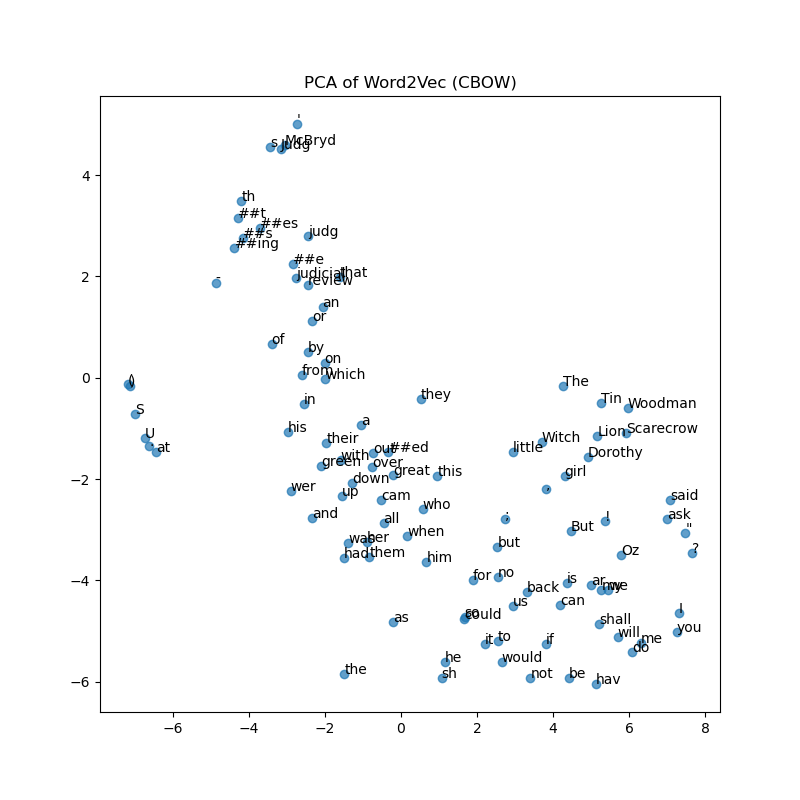
\includegraphics[width=0.49\textwidth]{cbow.png}
    \hfill
    % Second image
    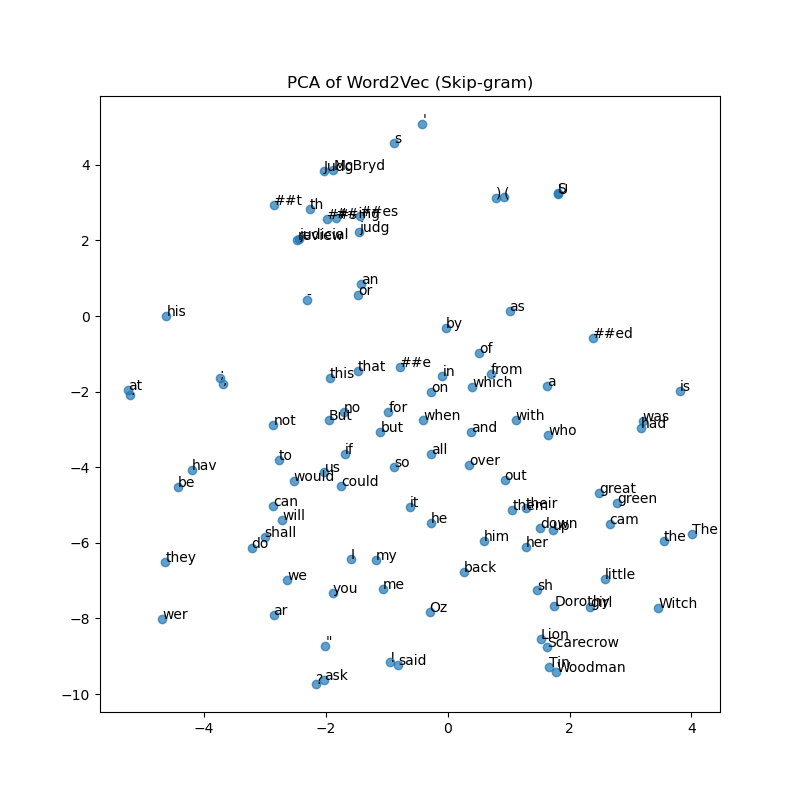
\includegraphics[width=0.49\textwidth]{skip-gram.png}
    \caption{PCA Analysis of Similarity Between Embedding Models}
    \label{fig:two-images-side-by-side}
\end{figure}

\section*{Conclusion}
The analysis indicates that both models recognize domain differences and achieve meaningful clustering of legal versus literary terminology. However, the largest divergences in similarity scores frequently involve tokens that are rare or partial. CBOW, which predicts a word from an average of surrounding words, can inflate similarity for such tokens if they regularly co-occur with certain frequent words or appear in varied contexts. Skip-gram, in contrast, relies on individual \((\text{target}, \text{context})\) pairs and may assign negative similarities when two tokens hardly share direct contexts. Through examining the largest disparities, we see that the choice of architecture shapes how infrequent or partially tokenized words are embedded relative to more common terms.

Overall, the side-by-side comparison of CBOW and Skip-gram embeddings underscores each architecture's strengths and limitations in handling low-frequency items and subword tokens. The most substantial difference emerged in precisely those contexts where CBOW's averaging mechanism overrode nuanced distinctions that Skip-gram captured more distinctly.

\end{document}
